\documentclass[spanish]{article}
\usepackage{graphicx}
\usepackage{ragged2e}
\usepackage{geometry}
\usepackage{float}
\usepackage{hyperref}
\usepackage[table,xcdraw]{xcolor}
\usepackage[ruled,vlined]{algorithm2e}
\title {Práctica 5: Algoritmos Greedy}
\graphicspath{{../img/}}
\addtolength{\textheight}{1.5in} 
\begin{document}
	\centerline{
\includegraphics[width=450px,height=100px]{header}}
	\centerline{Analisis de algoritmos, Sem: 2021-1, 3CV1,Práctica  5, 11/12/2020}
	\centering{\huge{Práctica 5: Algoritmos Greedy}}
	\centerline{\newline{\textbf{Payán Téllez René}}}
	\newline{\textit{rpayant1500@alumno.ipn.mx}}
	\bigskip
	\justify
	\textbf{Resumen:}	
	En esta practica se analizaran 2 algoritmos que utilizan la tecnica de divide y venceras para resolver un problema, uno de ellos el quick sort y otro el sub arreglo maximo.\\
	\textbf{Palabras clave:}
	Huffman, Kruskal, Gredy, STL, C/C++
	\section{Introduccion}
	Los algoritmos glotones, son en su mayoria utilizados para resolver problemas extremadamente complejos de forma simple de programar, normalmente no es la mejor solucion pero casi siempre bastante cercana y se programa de forma extremadamente rapida, sin mencionar que normalmente no toman mucha complejidad computacional.
	Por ello aprender respecto a estos algoritmos es extremadamente importante, inclusive de los 2 que vamos a hablar a continuacion, ya que tienen usos tanto en redes (Huffman) como en proyectos (Kruskal).
	\section{Conceptos Basicos}
	\subsection{Algoritmo}
		La palabra algoritmo proviene del sobrenombre de un matemático árabe del siglo IX, Al-Khwarizmi, que fue reconocido por enunciar paso a paso las reglas para las operaciones matemáticas básicas con decimales (suma, resta, multiplicación y división).	
		Vemos definición de algoritmo como un grupo de órdenes consecutivas que presentan una solución a un problema o tarea. Algunos ejemplos de algoritmos los podemos encontrar en las matemáticas (como el algoritmo para resolver una multiplicación) y en los manuales de usuario de un aparato (como una lavadora o una impresora).	
		Sin embargo, hoy en día se relaciona la palabra algoritmo con el mundo de la informática, más concretamente en la programación; los conocidos como algoritmos informáticos.[1]
	\subsection{Complejidad algoritmica}
		Así que, por su naturaleza, un problema tiene la capacidad de ser solucionado por uno o varios métodos, pero si bien es importante llegar a la respuesta, más importante es evaluar su viabilidad. Siempre que se analiza y evalúa adecuadamente la efectividad de una solución, disminuye drásticamente el costo que representa su producción y mantenimiento, pues los recursos que se invierten posteriormente en codificación, pruebas y revisión es mucho menor siempre (como el tiempo, dinero y talento humano).	
		Entrando en materia, la complejidad algorítmica es una métrica teórica que nos ayuda a describir el comportamiento de un algoritmo en términos de tiempo de ejecución (tiempo que tarda un algoritmo en resolver un problema) y memoria requerida (cantidad de memoria necesaria para procesar las instrucciones que solucionan dicho problema). Esto nos ayuda a comparar entre la efectividad de un algoritmo y otro, y decidir cuál es el que nos conviene implementar.[2]
	\subsection{Algoritmos Greedy o glotones}	
		Un algoritmo Greedy o gloton es un algoritmo muy util para encontrar soluciones aproximadas e inclusive la mas optima a problemas complejos, ya que las entregan en muy corto tiempo. Se llaman Greedy porque siempre "comen lo que tienen a la mano", no garantizan encontrar la mejor solucion, pero si una aproximacion bastante buena.[3]
		Estas son sus caracteristicas principales:
		\begin{itemize}
			\item Se utilizan generalmente para resolver problemas deoptimización (obtener el máximo o el mínimo).optimización (obtener el máximo o el mínimo).
			\item Toman decisiones en función de la información que está disponible en cada momento. está disponible en cada momento. está disponible en cada momento. está disponible en cada momen
			\item Una vez tomada la decisión, ésta no vuelve a replantearse en el futuro.replantearse en el futuro.
			\item Suelen ser rápidos y fáciles de implementar.
			\item No siempre garantizan alcanzar la solución óptima[4]
		\end{itemize}
	\subsection{Algoritmo de codificación de Huffman}
		El código de Huffman es un tipo particular de código de prefijo óptimo que se usa comúnmente para la compresión de datos sin pérdida. Comprime los datos de manera muy efectiva, ahorrando de 20$\%$ a 90$\%$ de memoria, dependiendo de las características de los datos comprimidos. Este algoritmo se aplica solo si se considera a la entrada como una cadena de caracteres, ya que es un algoritmo boraz que utiliza una tabla que proporciona la frecuencia con la que aparece cada carácter (es decir, su frecuencia) para crear una forma óptima de representar cada carácter como una cadena binaria. Fue propuesto por David A. Huffman en 1951.[5]\\
		\begin{algorithm}[H]
			\KwData{Entrada: C (Los caracteres de la cadena a codificar y su ocurrencia)}
			\KwResult{Retorna el arbol de huffman de la cadena}
			n = C.size\;
			Q = priority\_queue()\;
			\For{$i\gets 0$ \KwTo $i < n$}{
				n=node(C[i])\;
				Q.push(n)\;
			}
			\While{Q.size()$>$1}{
				Z = new node()\;
				Z.left = x = Q.pop()\;
				Z.right = y = Q.pop()\;
				Z.frequency = x.frequency+y.frequency\;
				Q.push(Z)\;
				
			}
			return Q\;
			\caption{HuffmanTree(C)}
		\end{algorithm}
		\begin{algorithm}[H]
			\KwData{Entrada: tree (El arbol de Huffman), S (la cadena binaria a descomprimir)}
			\KwResult{Retorna una cadena de caracteres descomprimida}
			n = S.length\;
			retorno = ""\;
			\For{$i\gets 0$ \KwTo $i < n$}{
				current = root\;
				\While{current.left != NULL and current.right!=NULL}{
					\If{S[i] == '0'}{
						current = current.left\;					
					}
					\Else{
						current = current.right\;											
					}				
					i+=1\;
				}
				retorno+=current.symbol\;
			}
			return retorno\;
			\caption{HuffmanDecompression(tree, S)}
		\end{algorithm}				
		\subsection{Algoritmos de Kruskal}			
			El algoritmo de Kruskal es un algoritmo de la teoría de grafos para encontrar un árbol recubridor mínimo en un grafo conexo y ponderado. Es decir, busca un subconjunto de aristas que, formando un árbol, incluyen todos los vértices y donde el valor de la suma de todas las aristas del árbol es el mínimo. Si el grafo no es conexo, entonces busca un bosque expandido mínimo (un árbol expandido mínimo para cada componente conexa).[6]\\ 
			Kruskal funciona de la siguiente forma:\\
			\begin{enumerate}
				\item     Se selecciona, de entre todas las aristas restantes, la de menor peso siempre que no cree ningún ciclo.
				\item Se repite el paso 1 hasta que se hayan seleccionado $\|V\| - 1$ aristas.[7]
			\end{enumerate}
			\begin{algorithm}[H]
				\KwData{Entrada: G (un grafo)}
				\KwResult{Retorna el arbol de extencion minima}
				\ForEach{v \KwTo V[G]}{
					Z = union\_find(C[v]\KwTo {v})\;
				}
				Q = priority\_queue(A[G])\;
				T = new Tree()\;
				\While{ A[T] $\leq$ n-1 and !Q.empty()}{
					(u,v) \KwTo Q.sacarMin();
					\If{C(v) $\neq$ C(u)}{
						T.push((u,v))\;
						Merge(C(v), C(u))\;
					}
				}
				return T\;
			\end{algorithm}	
			Su complejidad es $O(mlog_2(n))$[8], donde m es el numero de aristas y n el numero de nodos.
	\section{Experimentacion y Resultados}
	\subsection{Implementar el algoritmo de codificacion de Huffman.}
	Para esta primera parte de pruebas se implemento el algoritmo de codificacion y decodificacion de Huffman, asi que la ejecución se divide en 2 partes, la compresion de una cadena de texto y para la segunda parte la descompresion de la misma
	\begin{figure}[H]
		\centering
		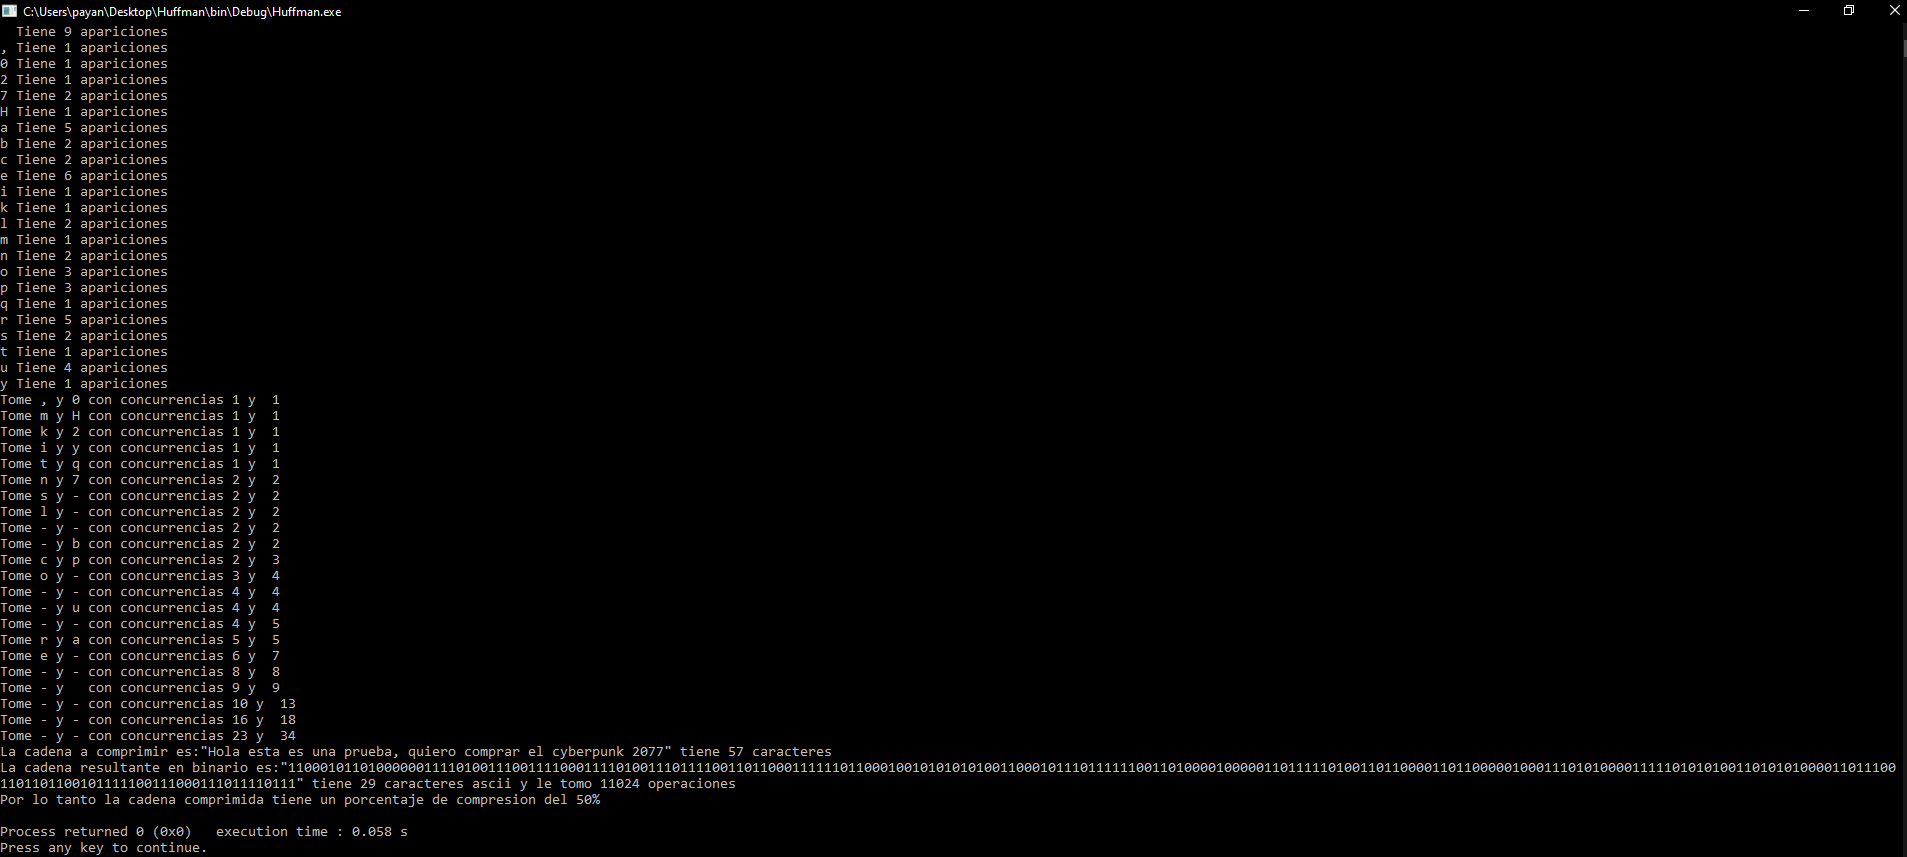
\includegraphics[width=400px,height=300px]{captura1}
		\caption{Compresión de la cadena "Hola esta es una prueba, quiero comprar el cyberpunk 2077"}
	\end{figure}
	
	\begin{figure}[H]
		\centering
		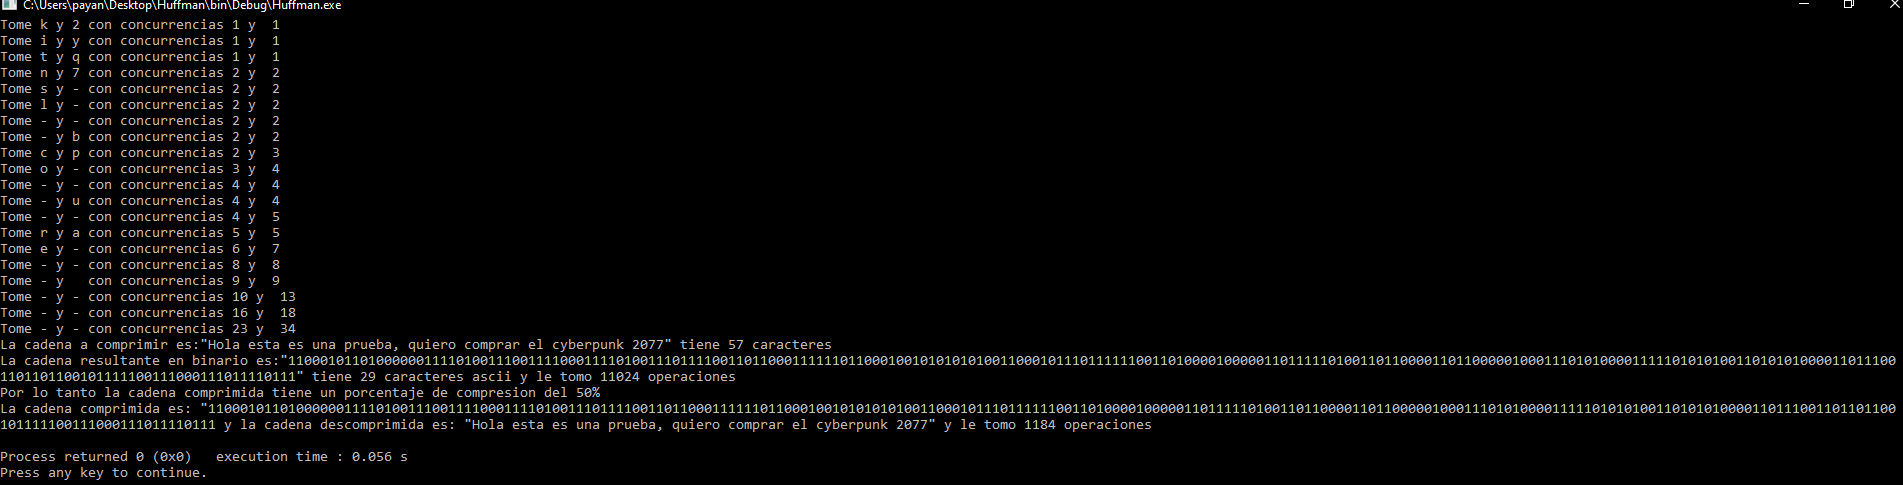
\includegraphics[width=400px,height=300px]{captura2}
		\caption{Descompresión  de la cadena "Hola esta es una prueba, quiero comprar el cyberpunk 2077"}
	\end{figure}
	Como se pudo apreciar en las capturas, la capturas, el programa tomo la entrada "Hola esta es una prueba, quiero comprar el cyberpunk 2077" y retorno la siguiente salida como respuesta: "", posteriormente al introducir la salida de la compresion en la seccion de descompresion, el programa arrojo la cadena original.
	Podemos decir que el algoritmo es eficiente, porque esta es la cantidad de caracteres de la cadena original:
	\begin{figure}[H]
		\centering
		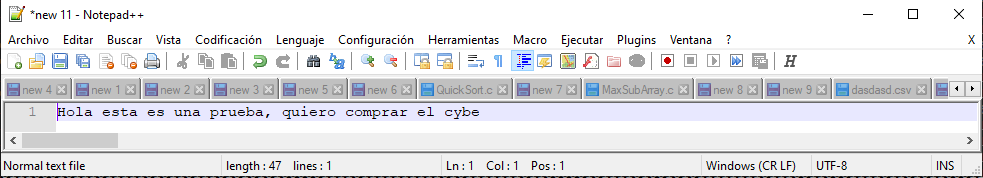
\includegraphics[width=400px,height=150px]{captura3}
		\caption{Conteo de caracteres de la entrada}
	\end{figure}
	esta es la cantidad de caracteres de la salida:
	\begin{figure}[H]
		\centering
		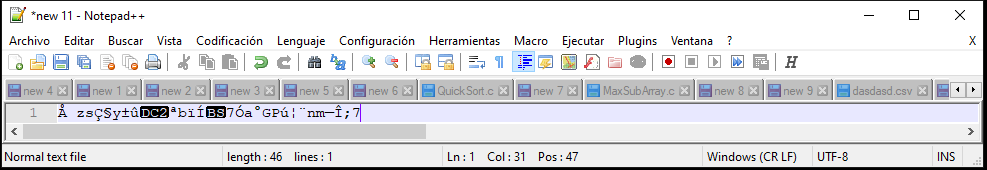
\includegraphics[width=400px,height=150px]{captura4}
		\caption{Conteo de caracteres de la salida}
	\end{figure}
	por ultimo, el binario de cada caracter asignado
	\begin{figure}[H]
		\centering
		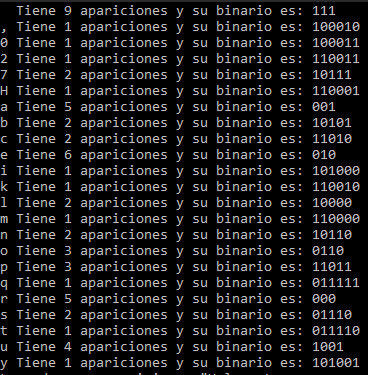
\includegraphics[width=400px,height=300px]{captura9}
		\caption{Asignacion de binario}
	\end{figure}
	A continuacion se probo con una cadena mas larga, un "Lorem Ipsum" de 1000 bytes:
	Lorem ipsum dolor sit amet, consectetur adipiscing elit. Integer porttitor turpis eget erat auctor varius. Vestibulum maximus scelerisque dui ac vulputate. Mauris eleifend mauris vel ex sodales, ut blandit odio dictum. Ut efficitur eu lectus nec ullamcorper. Integer hendrerit justo in augue consectetur, eget porttitor quam rutrum. Cras porta justo at fermentum condimentum. Nunc lacinia convallis tortor in tempor. Donec tincidunt tempor ipsum, sit amet aliquet justo semper at. Donec nibh urna, faucibus ac mauris eu, mattis imperdiet dolor. Nam et nulla at nisi efficitur efficitur. Morbi bibendum scelerisque risus, at sollicitudin ligula rutrum et. Cras sagittis eget velit aliquam cursus.
	Nunc magna metus, ullamcorper sed ante id, tincidunt ornare libero. Proin pharetra orci felis, eget pellentesque nisi venenatis eget. Morbi tincidunt ut risus non iaculis. Proin id consectetur metus, sed placerat eros. Aenean cursus augue a ipsum tempor interdum. Vivamus viverra efficitur felis a aenean. 
	\begin{figure}[H]
		\centering
		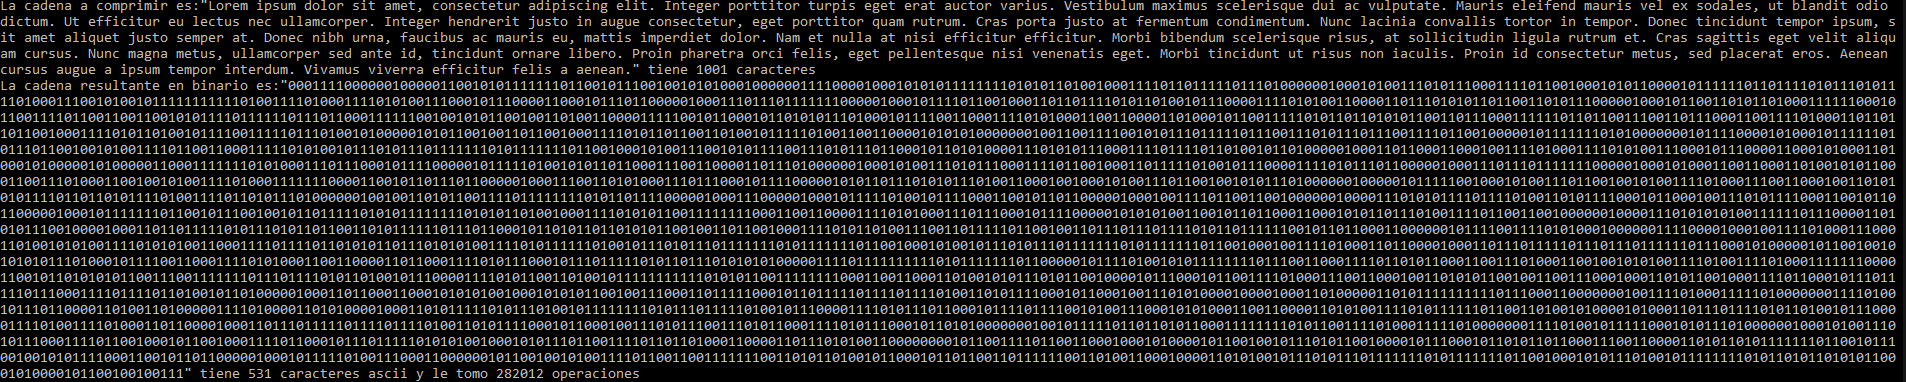
\includegraphics[width=400px,height=300px]{captura5}
		\caption{Compresión del lorem ipsum}
	\end{figure}
	
	\begin{figure}[H]
		\centering
		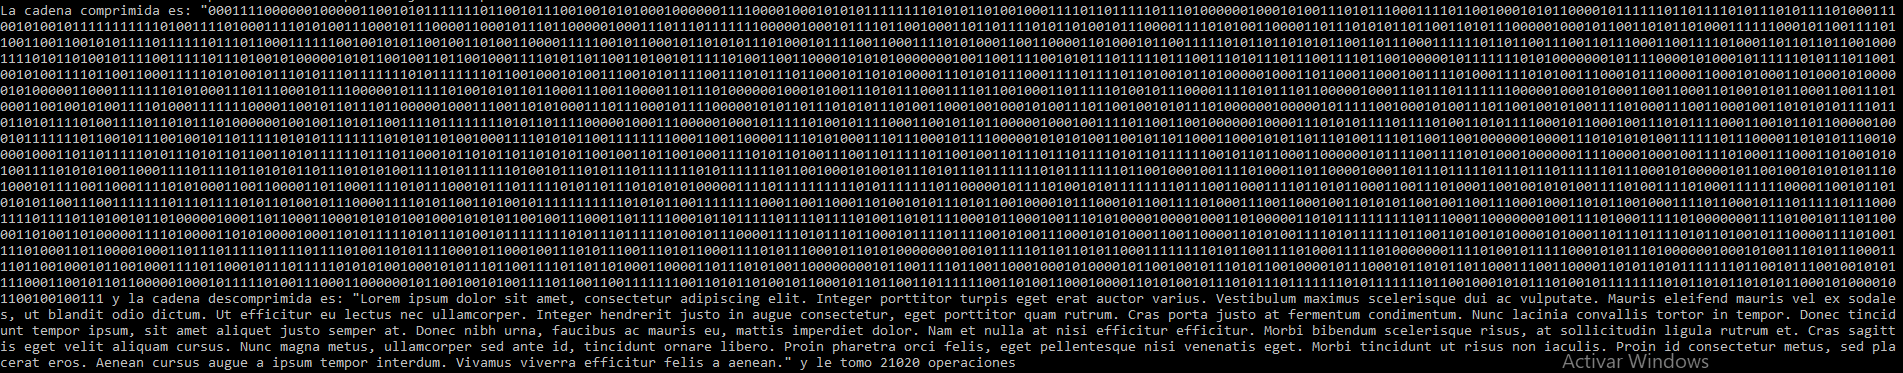
\includegraphics[width=400px,height=300px]{captura6}
		\caption{Descompresión del lorem ipsum}
	\end{figure}
	Finalmente se contaron los caractres de la entrada y de la salida:
	\begin{figure}[H]
		\centering
		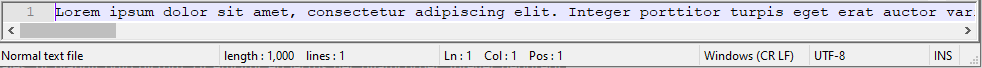
\includegraphics[width=400px,height=150px]{captura7}
		\caption{Conteo de caracteres de la entrada}
	\end{figure}
	y esta es la cantidad de caracteres de la salida:
	\begin{figure}[H]
		\centering
		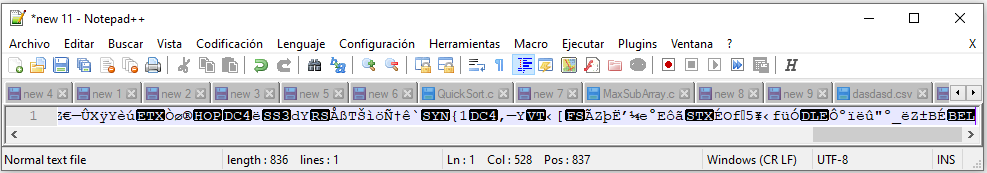
\includegraphics[width=400px,height=150px]{captura8}
		\caption{Conteo de caracteres de la salida}
	\end{figure}
	por ultimo, el binario de cada caracter asignado
	\begin{figure}[H]
		\centering
		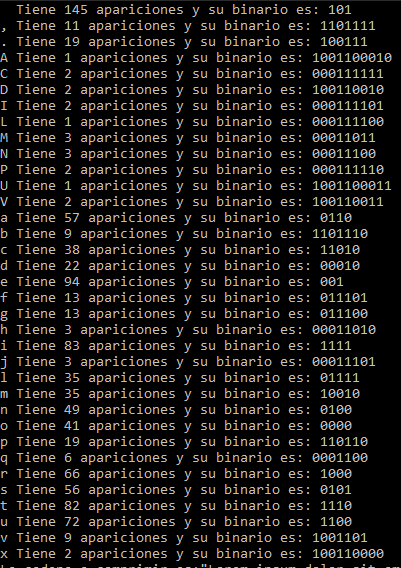
\includegraphics[width=400px,height=300px]{captura10}
		\caption{Asignacion de binario}
	\end{figure}
	A continuación se comprimieron 10 archivos de texto con extencion .txt de distinto tamaño, se anexan las capturas del binario de cada caracter, del archivo de entrada, el archivo comprimido, el archivo descomprimido y el tamaño de ambos archivos.\\
	\textbf{Primer archivo}
	\begin{figure}[H]
		\centering
		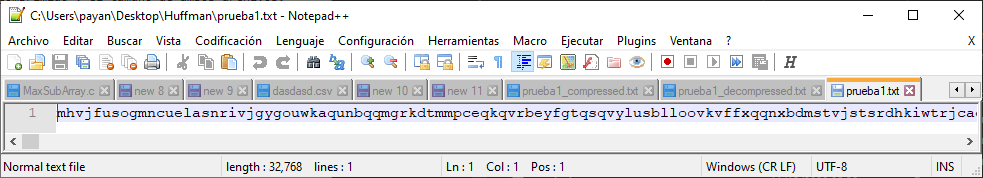
\includegraphics[width=400px,height=150px]{captura11}
		\caption{Archivo de entrada}
	\end{figure}
	\begin{figure}[H]
		\centering
		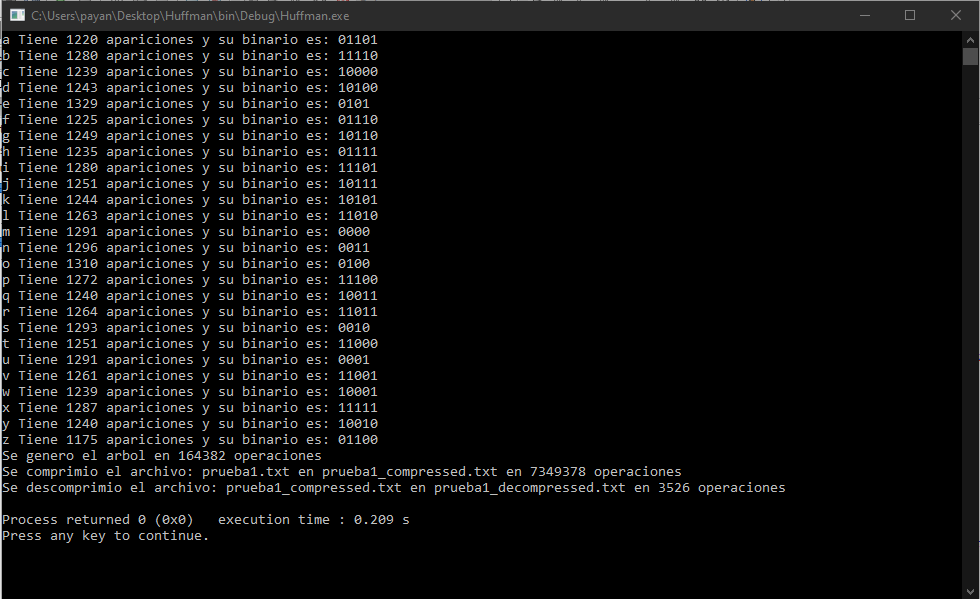
\includegraphics[width=400px,height=300px]{captura12}
		\caption{Ejecucion del programa}
	\end{figure}
	\begin{figure}[H]
		\centering
		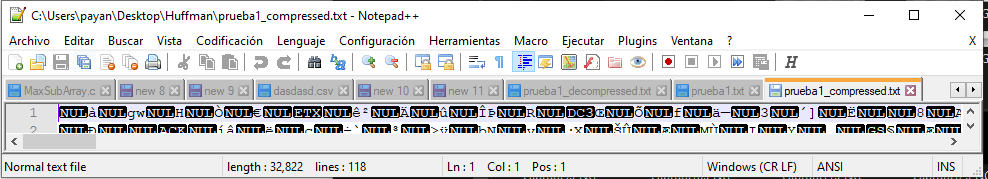
\includegraphics[width=400px,height=150px]{captura13}
		\caption{Archivo de salida}
	\end{figure}
	\begin{figure}[H]
		\centering
		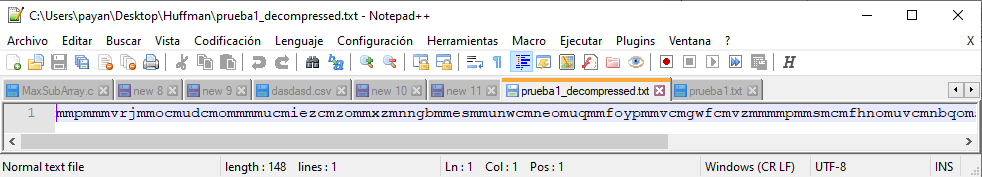
\includegraphics[width=400px,height=150px]{captura14}
		\caption{Archivo descomprimido}
	\end{figure}
	\begin{figure}[H]
		\centering
		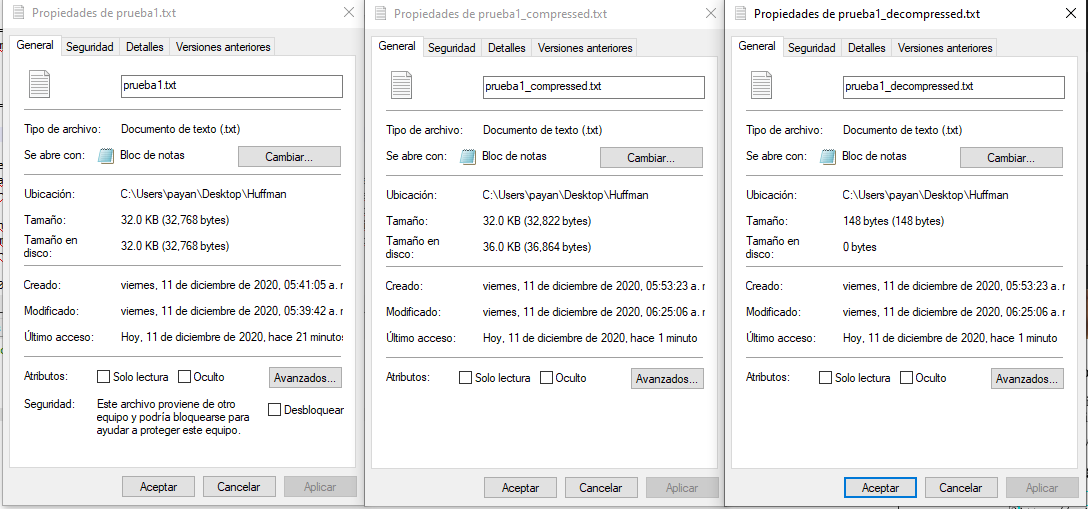
\includegraphics[width=400px,height=150px]{captura15}
		\caption{peso de los 3 archivos}
	\end{figure}
	\textbf{Segundo archivo}
	\begin{figure}[H]
		\centering
		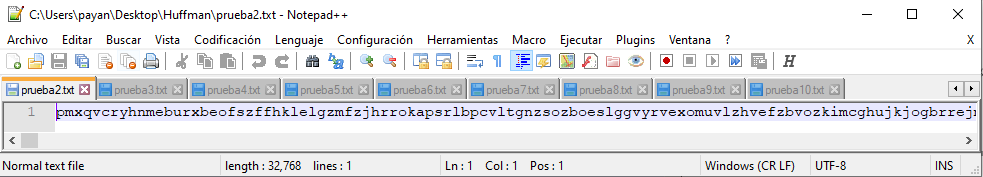
\includegraphics[width=400px,height=150px]{captura16}
		\caption{Archivo de entrada}
	\end{figure}
	\begin{figure}[H]
		\centering
		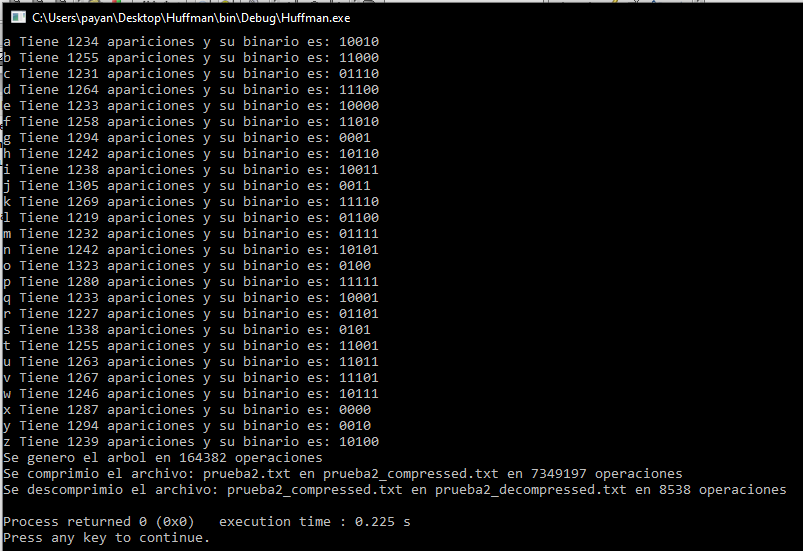
\includegraphics[width=400px,height=300px]{captura17}
		\caption{Ejecucion del programa}
	\end{figure}
	\begin{figure}[H]
		\centering
		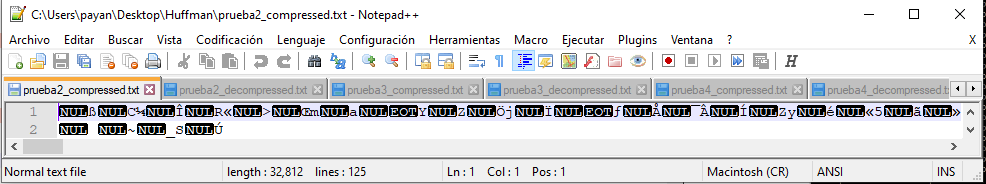
\includegraphics[width=400px,height=150px]{captura18}
		\caption{Archivo de salida}
	\end{figure}
	\begin{figure}[H]
		\centering
		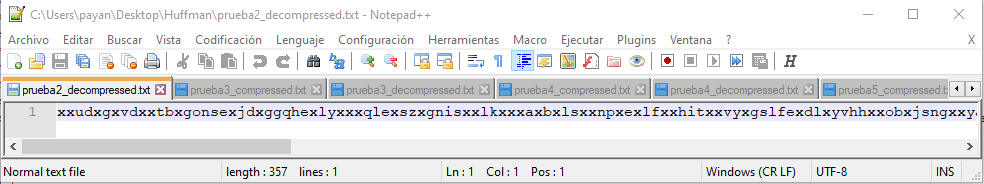
\includegraphics[width=400px,height=150px]{captura19}
		\caption{Archivo descomprimido}
	\end{figure}
	\begin{figure}[H]
		\centering
		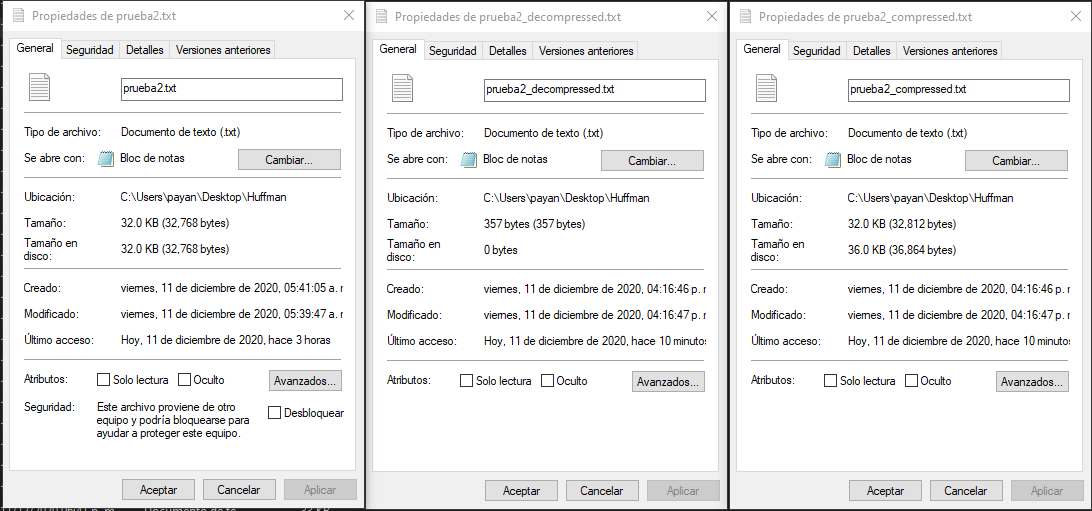
\includegraphics[width=400px,height=150px]{captura20}
		\caption{peso de los 3 archivos}
	\end{figure}
	\textbf{Tercer archivo}
	\begin{figure}[H]
		\centering
		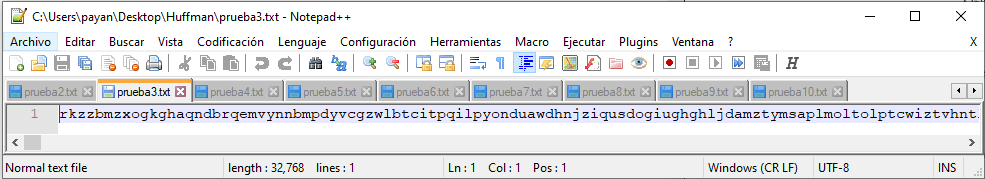
\includegraphics[width=400px,height=150px]{captura21}
		\caption{Archivo de entrada}
	\end{figure}
	\begin{figure}[H]
		\centering
		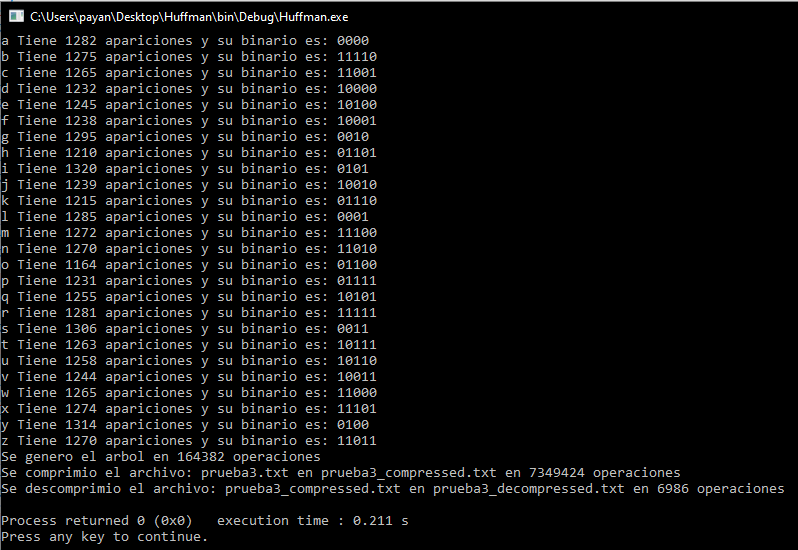
\includegraphics[width=400px,height=300px]{captura22}
		\caption{Ejecucion del programa}
	\end{figure}
	\begin{figure}[H]
		\centering
		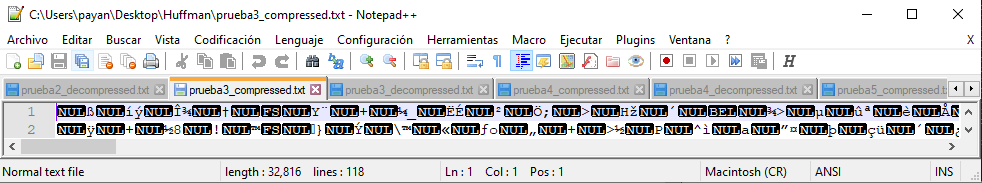
\includegraphics[width=400px,height=150px]{captura23}
		\caption{Archivo de salida}
	\end{figure}
	\begin{figure}[H]
		\centering
		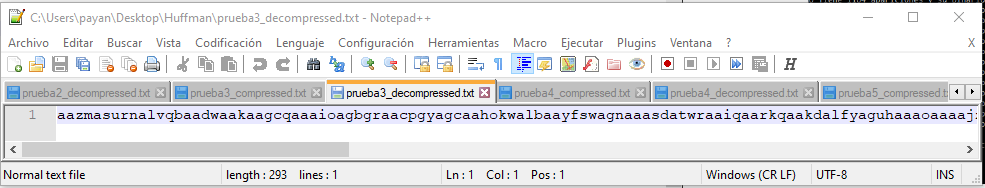
\includegraphics[width=400px,height=150px]{captura24}
		\caption{Archivo descomprimido}
	\end{figure}
	\begin{figure}[H]
		\centering
		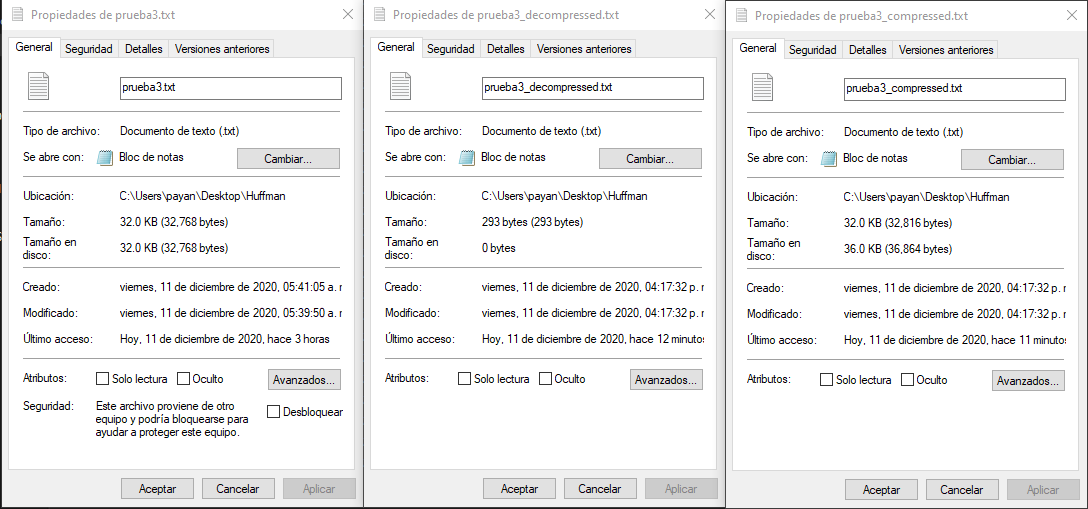
\includegraphics[width=400px,height=150px]{captura25}
		\caption{peso de los 3 archivos}
	\end{figure}
	\textbf{Cuarto archivo}
	\begin{figure}[H]
		\centering
		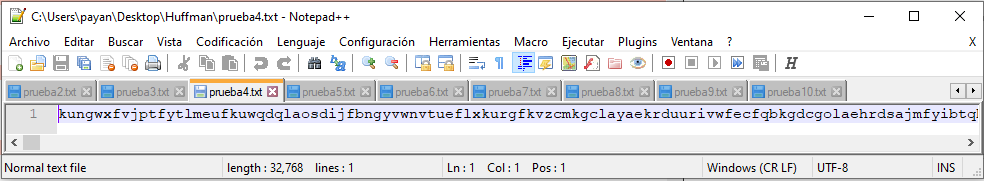
\includegraphics[width=400px,height=150px]{captura26}
		\caption{Archivo de entrada}
	\end{figure}
	\begin{figure}[H]
		\centering
		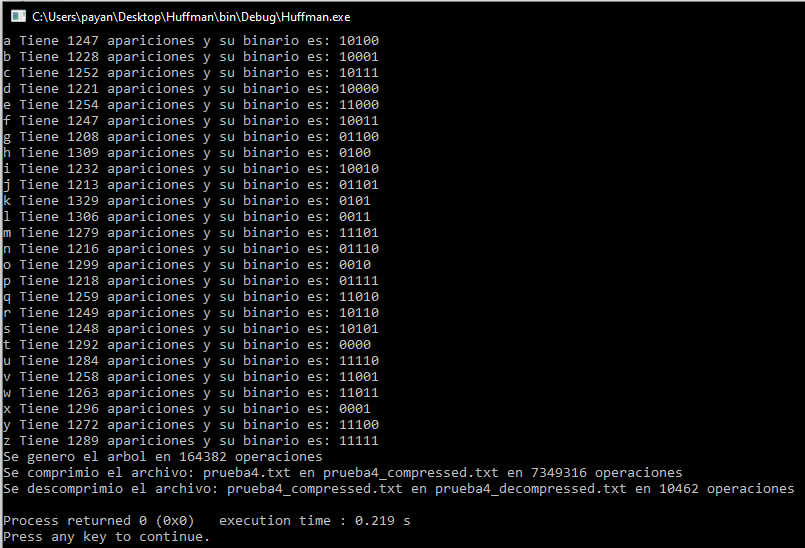
\includegraphics[width=400px,height=300px]{captura27}
		\caption{Ejecucion del programa}
	\end{figure}
	\begin{figure}[H]
		\centering
		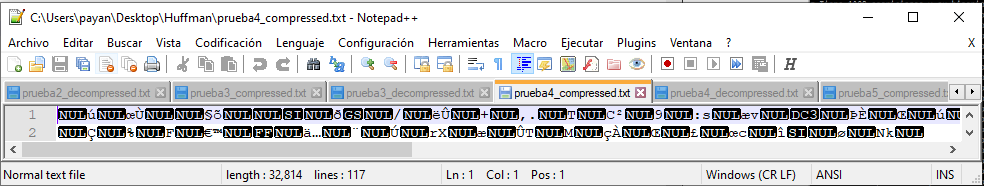
\includegraphics[width=400px,height=150px]{captura28}
		\caption{Archivo de salida}
	\end{figure}
	\begin{figure}[H]
		\centering
		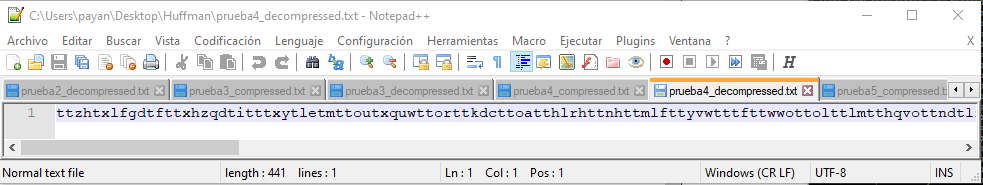
\includegraphics[width=400px,height=150px]{captura29}
		\caption{Archivo descomprimido}
	\end{figure}
	\begin{figure}[H]
		\centering
		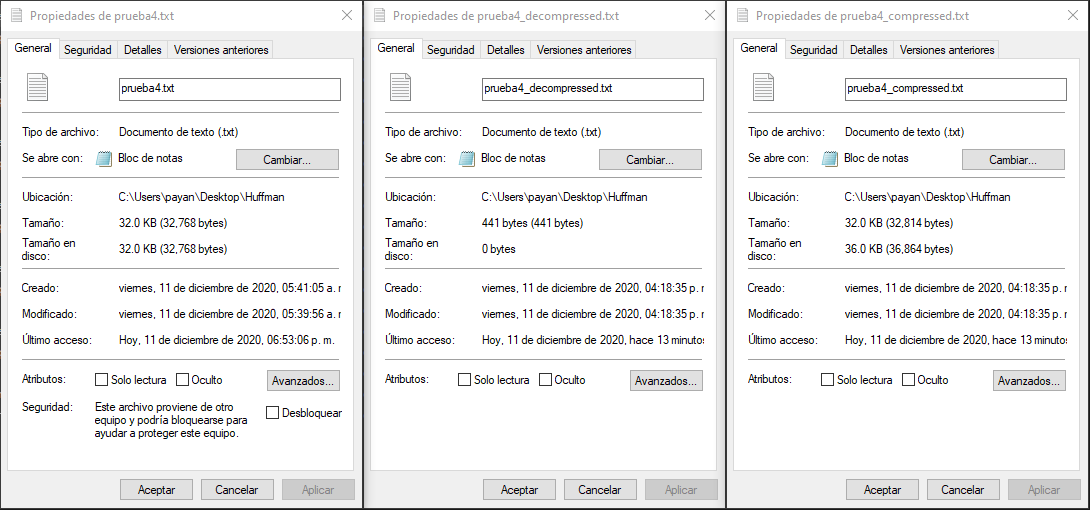
\includegraphics[width=400px,height=150px]{captura30}
		\caption{peso de los 3 archivos}
	\end{figure}
	\textbf{Quinto archivo}
	\begin{figure}[H]
		\centering
		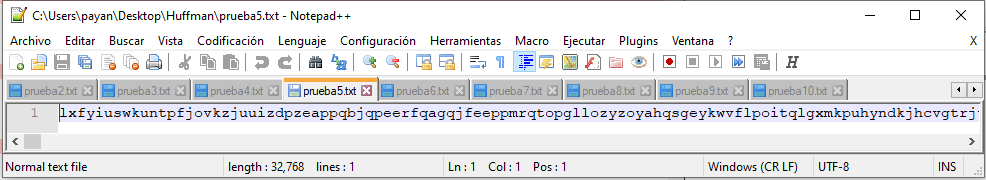
\includegraphics[width=400px,height=150px]{captura31}
		\caption{Archivo de entrada}
	\end{figure}
	\begin{figure}[H]
		\centering
		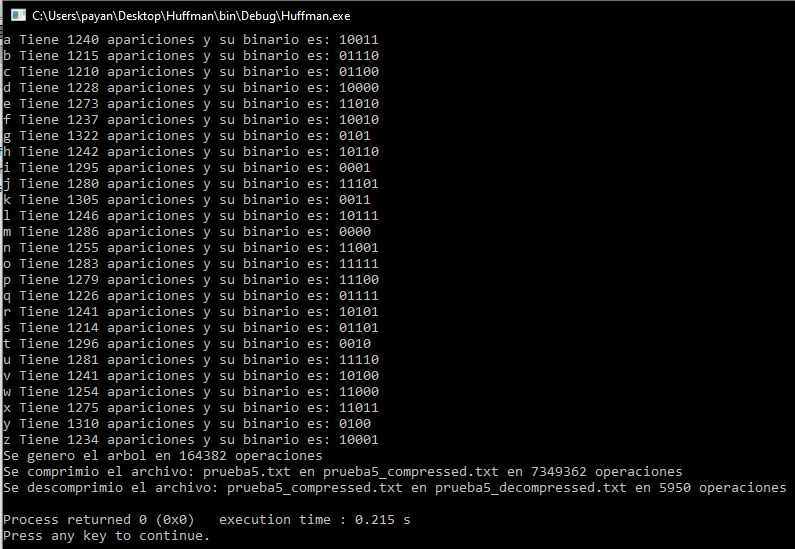
\includegraphics[width=400px,height=300px]{captura32}
		\caption{Ejecucion del programa}
	\end{figure}
	\begin{figure}[H]
		\centering
		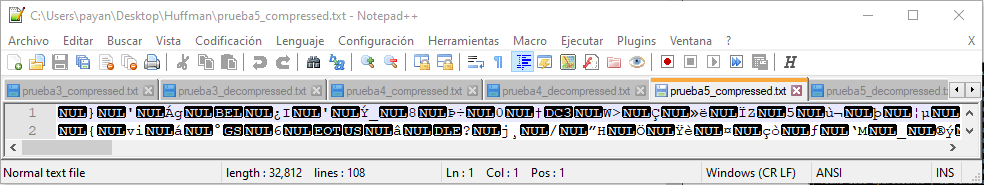
\includegraphics[width=400px,height=150px]{captura33}
		\caption{Archivo de salida}
	\end{figure}
	\begin{figure}[H]
		\centering
		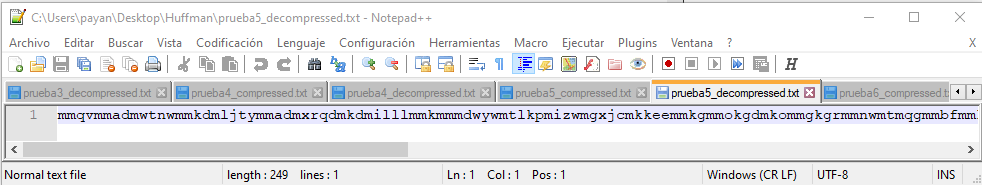
\includegraphics[width=400px,height=150px]{captura34}
		\caption{Archivo descomprimido}
	\end{figure}
	\begin{figure}[H]
		\centering
		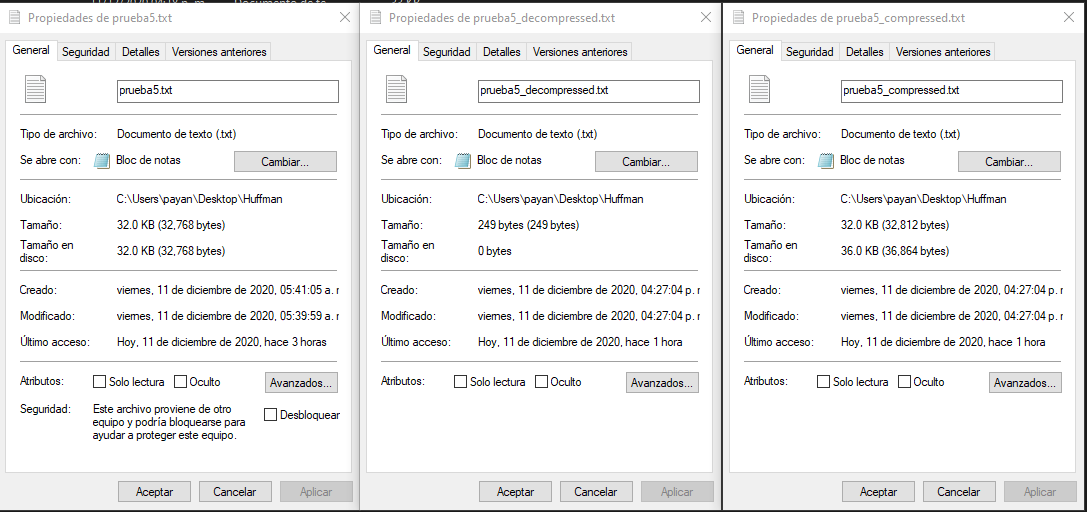
\includegraphics[width=400px,height=150px]{captura35}
		\caption{peso de los 3 archivos}
	\end{figure}
	\textbf{Sexto archivo}
	\begin{figure}[H]
		\centering
		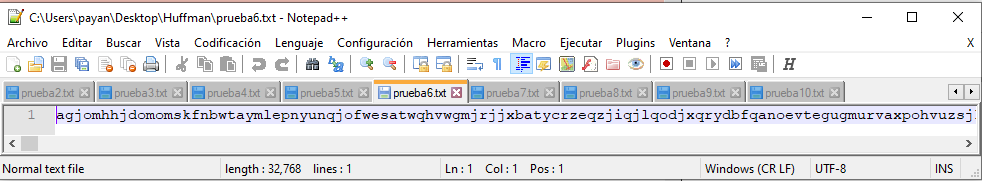
\includegraphics[width=400px,height=150px]{captura36}
		\caption{Archivo de entrada}
	\end{figure}
	\begin{figure}[H]
		\centering
		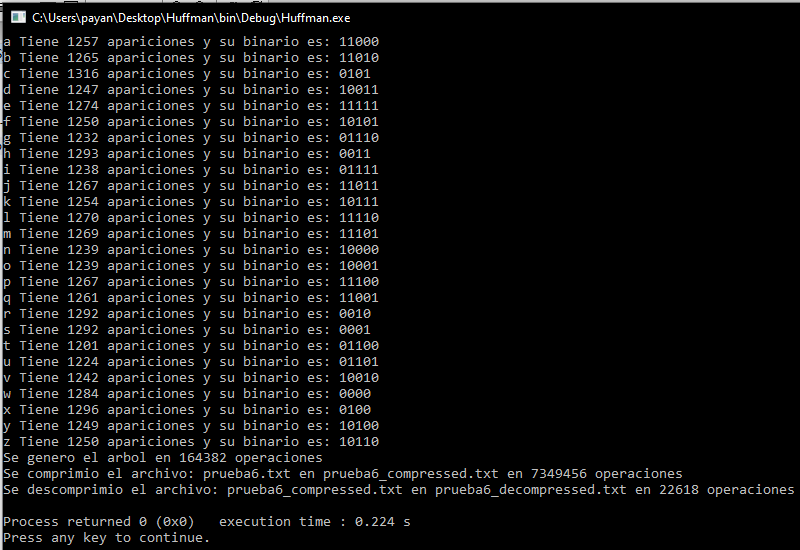
\includegraphics[width=400px,height=300px]{captura37}
		\caption{Ejecucion del programa}
	\end{figure}
	\begin{figure}[H]
		\centering
		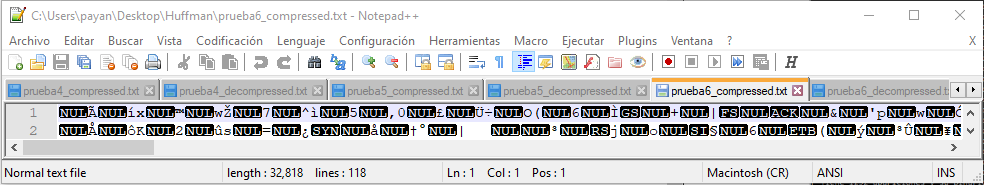
\includegraphics[width=400px,height=150px]{captura38}
		\caption{Archivo de salida}
	\end{figure}
	\begin{figure}[H]
		\centering
		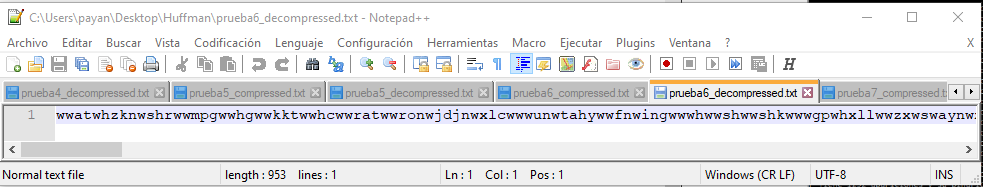
\includegraphics[width=400px,height=150px]{captura39}
		\caption{Archivo descomprimido}
	\end{figure}
	\begin{figure}[H]
		\centering
		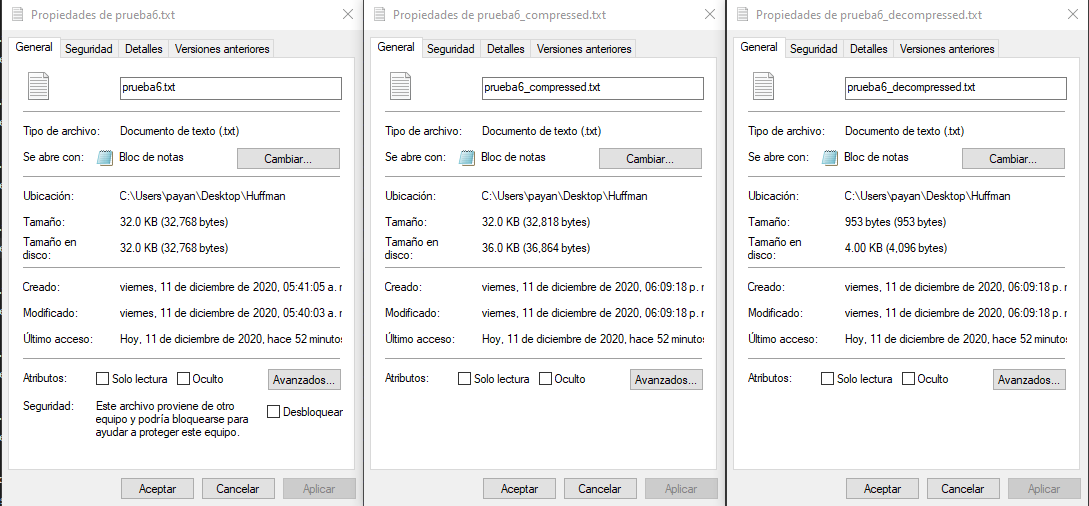
\includegraphics[width=400px,height=150px]{captura40}
		\caption{peso de los 3 archivos}
	\end{figure}
	\textbf{Septimo archivo}
	\begin{figure}[H]
		\centering
		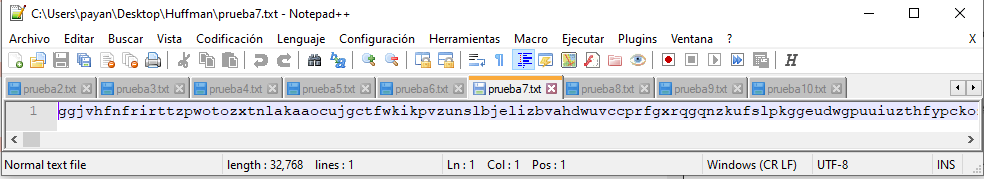
\includegraphics[width=400px,height=150px]{captura41}
		\caption{Archivo de entrada}
	\end{figure}
	\begin{figure}[H]
		\centering
		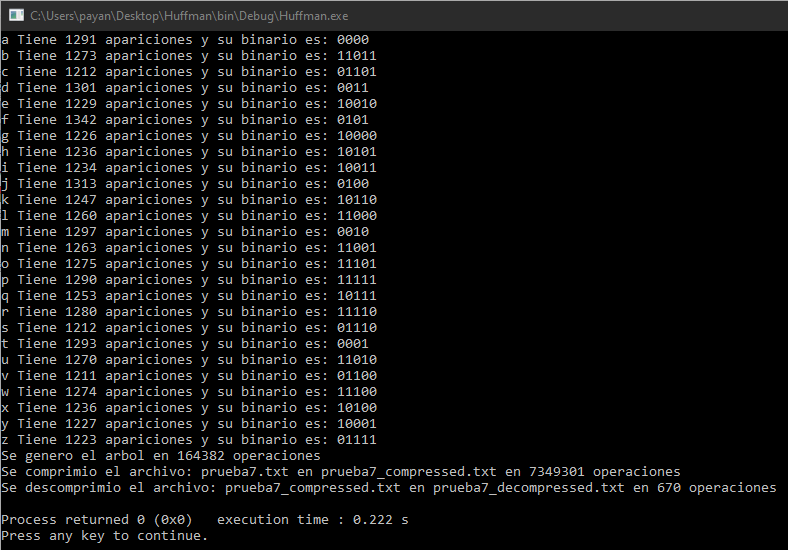
\includegraphics[width=400px,height=300px]{captura42}
		\caption{Ejecucion del programa}
	\end{figure}
	\begin{figure}[H]
		\centering
		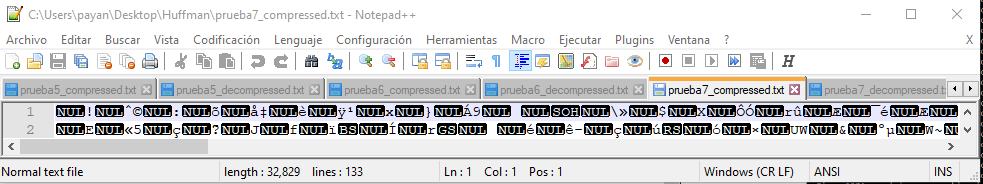
\includegraphics[width=400px,height=150px]{captura43}
		\caption{Archivo de salida}
	\end{figure}
	\begin{figure}[H]
		\centering
		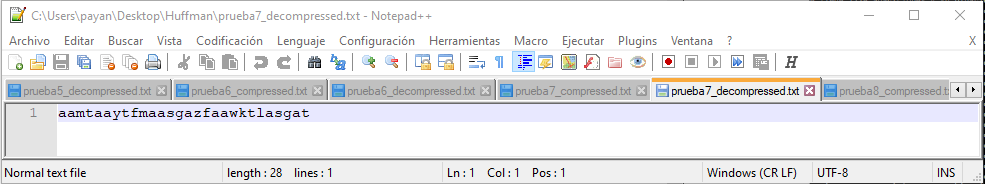
\includegraphics[width=400px,height=150px]{captura44}
		\caption{Archivo descomprimido}
	\end{figure}
	\begin{figure}[H]
		\centering
		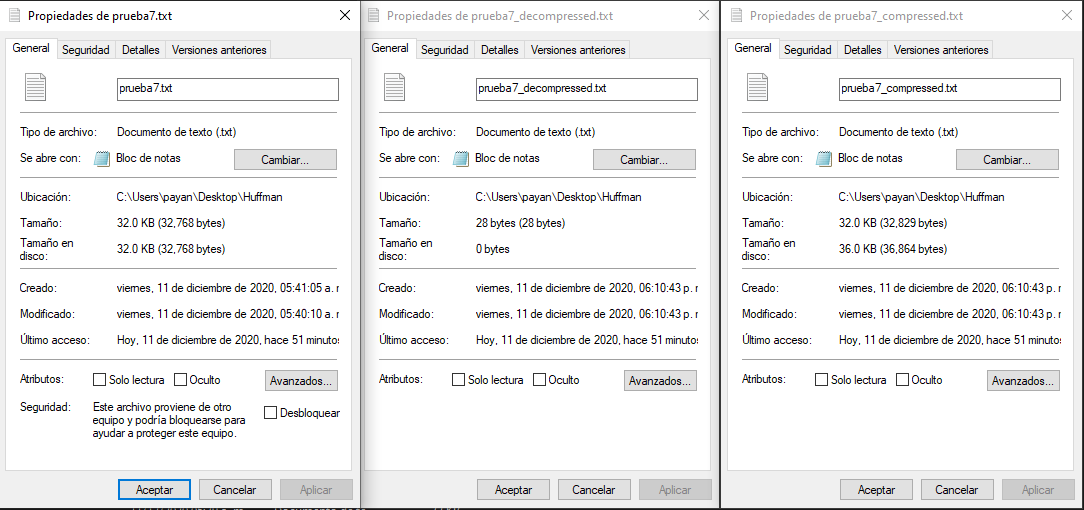
\includegraphics[width=400px,height=150px]{captura45}
		\caption{peso de los 3 archivos}
	\end{figure}
	\textbf{Octavo archivo}
	\begin{figure}[H]
		\centering
		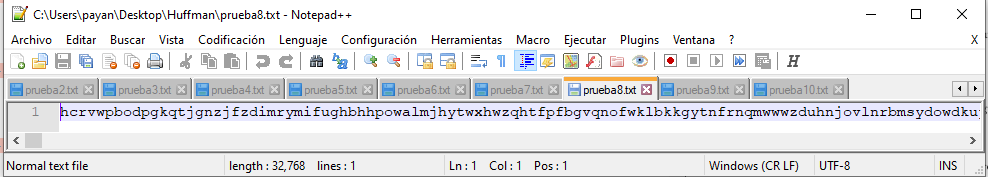
\includegraphics[width=400px,height=150px]{captura46}
		\caption{Archivo de entrada}
	\end{figure}
	\begin{figure}[H]
		\centering
		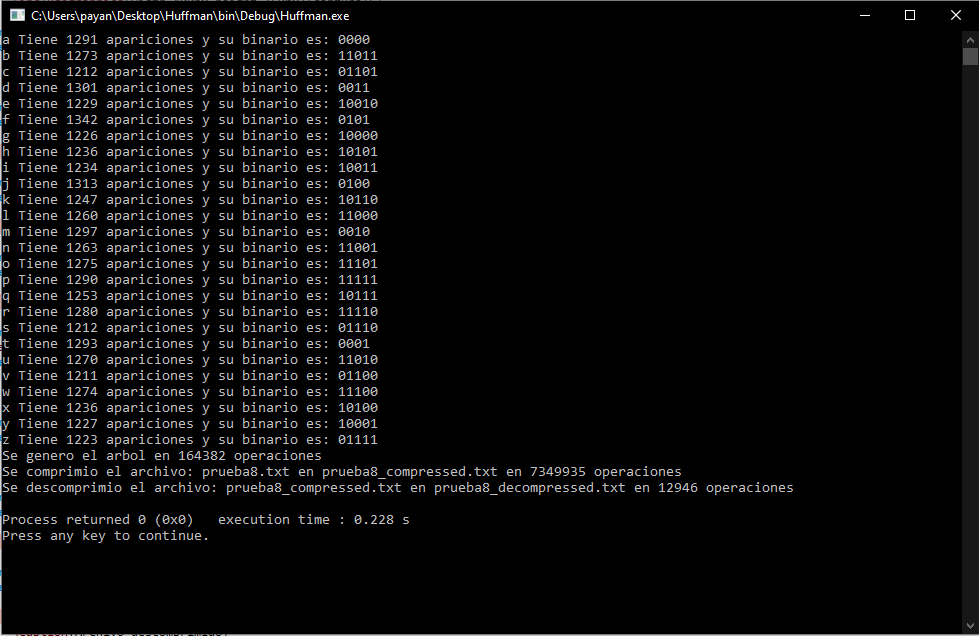
\includegraphics[width=400px,height=300px]{captura47}
		\caption{Ejecucion del programa}
	\end{figure}
	\begin{figure}[H]
		\centering
		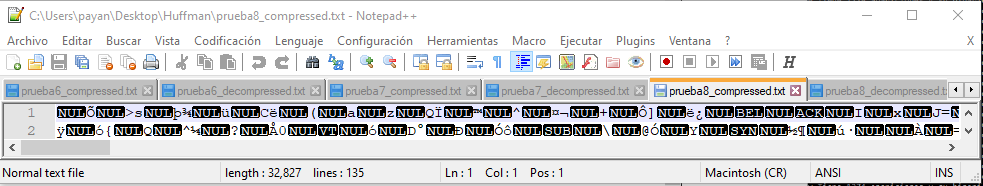
\includegraphics[width=400px,height=150px]{captura48}
		\caption{Archivo de salida}
	\end{figure}
	\begin{figure}[H]
		\centering
		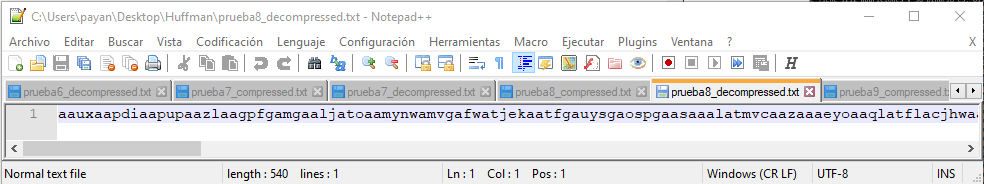
\includegraphics[width=400px,height=150px]{captura49}
		\caption{Archivo descomprimido}
	\end{figure}
	\begin{figure}[H]
		\centering
		\includegraphics[width=400px,height=150px]{captura50}
		\caption{peso de los 3 archivos}
	\end{figure}
	\textbf{Noveno archivo}
	\begin{figure}[H]
		\centering
		\includegraphics[width=400px,height=150px]{captura51}
		\caption{Archivo de entrada}
	\end{figure}
	\begin{figure}[H]
		\centering
		\includegraphics[width=400px,height=300px]{captura52}
		\caption{Ejecucion del programa}
	\end{figure}
	\begin{figure}[H]
		\centering
		\includegraphics[width=400px,height=150px]{captura53}
		\caption{Archivo de salida}
	\end{figure}
	\begin{figure}[H]
		\centering
		\includegraphics[width=400px,height=150px]{captura54}
		\caption{Archivo descomprimido}
	\end{figure}
	\begin{figure}[H]
		\centering
		\includegraphics[width=400px,height=150px]{captura55}
		\caption{peso de los 3 archivos}
	\end{figure}
	\textbf{Decimo archivo}
	\begin{figure}[H]
		\centering
		\includegraphics[width=400px,height=150px]{captura56}
		\caption{Archivo de entrada}
	\end{figure}
	\begin{figure}[H]
		\centering
		\includegraphics[width=400px,height=300px]{captura57}
		\caption{Ejecucion del programa}
	\end{figure}
	\begin{figure}[H]
		\centering
		\includegraphics[width=400px,height=150px]{captura58}
		\caption{Archivo de salida}
	\end{figure}
	\begin{figure}[H]
		\centering
		\includegraphics[width=400px,height=150px]{captura59}
		\caption{Archivo descomprimido}
	\end{figure}
	\begin{figure}[H]
		\centering
		\includegraphics[width=400px,height=150px]{captura60}
		\caption{peso de los 3 archivos}
	\end{figure}
	Finalmente para concluir este algorimo, se realizo una modificacion al codigo para generar una cadena aleatoria de longitud "$n$", con (1$\leq n\leq 10000$), posteriormente a esta se le genero el arbol, se comprimio y descomprimio, para poder obtener la grafica de complejidad de los algorimos de compresion y descompresion de Huffman.
	\begin{figure}[H]
		\centering
		\includegraphics[width=400px,height=300px]{captura47}
		\caption{Ejecucion del programa generando cadenas aleatorias, comprimiendolas y descomprimiendolas}
	\end{figure}
	\begin{figure}[H]
		\centering
		\includegraphics[width=400px,height=300px]{grafica1}
		\caption{N contra operaciones de la generacion del arbol de Huffman}
	\end{figure}
	\begin{figure}[H]
		\centering
		\includegraphics[width=400px,height=300px]{grafica2}
		\caption{N contra operaciones de la codificacion de la cadena}
	\end{figure}
	\begin{figure}[H]
		\centering
		\includegraphics[width=400px,height=300px]{grafica3}
		\caption{N contra operaciones de la decodificacion de la cadena}
	\end{figure}
	\begin{figure}[H]
		\centering
		\includegraphics[width=400px,height=300px]{grafica4}
		\caption{N contra operaciones de la suma de la generacion del arbol de Huffman y compresion de la cadena}
	\end{figure}
	\begin{figure}[H]
		\centering
		\includegraphics[width=400px,height=300px]{grafica5}
		\caption{N contra operaciones de la suma de la generacion del arbol de Huffman y descompresion de la cadena}
	\end{figure}
	\begin{figure}[H]
		\centering
		\includegraphics[width=400px,height=300px]{grafica6}
		\caption{N contra operaciones de la suma de la generacion del arbol de Huffman, compresion y descompresion de la cadena}
	\end{figure}
	\begin{figure}[H]
		\centering
		\includegraphics[width=400px,height=300px]{grafica7}
		\caption{N contra operaciones comparando la generacion del arbol de Huffman y la compresion de datos}
	\end{figure}
	\begin{figure}[H]
		\centering
		\includegraphics[width=400px,height=300px]{grafica8}
		\caption{N contra operaciones comparando la generacion del arbol de Huffman y la descompresion de datos}
	\end{figure}
	\begin{figure}[H]
		\centering
		\includegraphics[width=400px,height=300px]{grafica9}
		\caption{N contra operaciones comparando la compresion y la descompresion de datos}
	\end{figure}
	\begin{figure}[H]
		\centering
		\includegraphics[width=400px,height=300px]{grafica10}
		\caption{N contra operaciones comparando la generacion del arbol de Huffman, la compresion de datos y la descompresion de los datos}
	\end{figure}
	Para realizar la comparacion correspondiente, se realiza el calculo de complejidad a priori usando el analisis linea a linea del pseudo codigo.
	primero la funcion \textbf{HuffmanTree(C)}
	\begin{center}
		\begin{table}[H]
			\begin{tabular}{|l|l|l|}
				\hline
				\rowcolor[HTML]{FFCC67} 
				Codigo                           & Costo & Veces ejecutado \\ \hline
				\textit{n = C.size()}                    & $\O(1)$    & 1               \\ \hline
				\textit{Q=priority\_queue()}                    & $\O(1)$    & 1               \\ \hline
				\textit{for(i=0;i$\leq$n;i++)} & $\O(n)$    & $n$+1             \\ \hline
				\textit{\  \  n=node(C[i])}                 & $\O(1)$    & $n$               \\ \hline
				\textit{\  \  Q.push(n)}                     & $\O(log_2(n-i))$    & $n$              \\ \hline
				\textit{while(Q.size()$>$1)} & $\O(log_2(n))$    & $log_2(n)+1$             \\ \hline
				\textit{\  \  z = new node()}                     & $\O(1)$    & $log_2(n)$               \\ \hline
				\textit{\  \  z.left = x = Q.pop()}                     & $\O(log_2(n))$    & $log_2(n)$               \\ \hline
				\textit{\  \  z.right = y = Q.pop()}                     & $\O(log_2(n))$    & $log_2(n)$               \\ \hline
				\textit{\  \  z.frequency = x.frequency+y.frequency}                     & $\O(1)$    & $log_2(n)$               \\ \hline
				\textit{\  \  Q.push(z)}                     & $\O(log_2(n))$    & $log_2(n)$               \\ \hline
				\textit{return Q.pop()}                     & $\O(1)$    & $1$               \\ \hline
			\end{tabular}
		\end{table}										
	\end{center}	
	Como podemos observar la mayor complejidad se encuentra dentro de los ciclos, donde en el peor escenario llega a ser $\O(nlog_2(n))$, considerando lo anterior se grafica la funcion $f(x) = xlog_2(x)$ y se anexa la grafica para ser comparada con los resultados del programa.
	\begin{figure}[H]
		\centering
		\includegraphics[width=400px,height=300px]{grafica11}
		\caption{Grafica de la funcion $f(x) = xlog_2(x)$  }
	\end{figure}
	Dada la grafica anterior, el analisis a posteriori y las graficas: Figure 62 y Figure 67, podemos concluir que la funcion para generar el arbol de Huffman tiene complejidad de $nlog_2(n)$\\
	Ahora se realiza el calculo de complejidad de la funcion \textbf{HuffmanDecompression(tree, S)}
	\begin{center}
		\begin{table}[H]
			\begin{tabular}{|l|l|l|}
				\hline
				\rowcolor[HTML]{FFCC67} 
				Codigo                           & Costo & Veces ejecutado \\ \hline
				\textit{n = S.length()}                    & $\O(1)$    & 1               \\ \hline
				\textit{retorno=""}                    & $\O(1)$    & 1               \\ \hline
				\textit{for(i=0;i$\leq$n;i++)} & $\O(n)$    & $n$+1             \\ \hline
				\textit{\  \  actual=tree}                 & $\O(1)$    & $n$               \\ \hline
				\textit{\  \  while(actual.left!=NULL and actual.right!=NULL)}                     & $\O(log_2(255))$    & $n$              \\ \hline
				\textit{\  \  \  \  if(S[i] == '0')} & $\O(1)$    & $log_2(255)*n$             \\ \hline
				\textit{\  \  \  \  \  \  actual = actual.left} & $\O(1)$    & $\frac{log_2(255)*n}{2}$             \\ \hline
				\textit{\  \  \  \  else} & $\O(1)$    & $log_2(255)*n$             \\ \hline
				\textit{\  \  \  \  \  \  actual = actual.right} & $\O(1)$    & $\frac{log_2(255)*n}{2}$             \\ \hline
				\textit{\  \  \  \  i++} & $\O(1)$    & $log_2(255)*n$             \\ \hline
				\textit{\  \  retorno+=actual.symbol} & $\O(1)$    & $n$             \\ \hline
				\textit{return retorno} & $\O(1)$    & $1$             \\ \hline				
			\end{tabular}
		\end{table}										
	\end{center}
	Entonces despues de analizar la funcion, podemos concluir que la funcion tiene complejdad $\O(n)$ siendo n la cantidad de bits en la cadena a descomprimir.
	\begin{figure}[H]
		\centering
		\includegraphics[width=400px,height=300px]{grafica12}
		\caption{Grafica de la funcion $f(x) = xlog_2(255)$  }
	\end{figure}
	Comparando la grafica de la funcion (Figure 73) y las graficas Figure 64, Figure 66, Figure 67, Figure 70, Figure 71, se verifica que la funcion tiene orden de complejidad lineal.
	\subsection{Implementar los algoritmos de Kruskal}
	Como ya conocemos la complejidad del algoritmo, no es necesario realizar el analisis a priori, por lo tanto graficamos directamente la complejidad $\O(mlog_2(n))$, considerando m = n.
	\begin{figure}[H]
		\centering
		\includegraphics[width=400px,height=300px]{grafica11}
		\caption{Grafica de la funcion $f(x) = xlog_2(x)$  }
	\end{figure}
	Ahora realizamos la implementacion del algoritmo para calcular su complejidad a posteriori. Se generan arboles aleatorios de n nodos y n aristas, donde (1$\leq n\leq 10000$) y graficamos la correspondiente informacion para validar la proposicion de complejidad.
	\begin{figure}[H]
		\centering
		\includegraphics[width=400px,height=300px]{captura62}
		\caption{Ejecucion del algoritmo programado}
	\end{figure}
	\begin{figure}[H]
		\centering
		\includegraphics[width=400px,height=300px]{grafica13}
		\caption{Grafica de n contra operaciones del algoritmo de Kruskal}
	\end{figure}
	\section{Conclusiones}			
	\subsection{Payán Téllez René}
	Durante el desarrollo de esta practica hubo muchas cosas inesperadas, como el hecho de que por usar la STL no se pudo medir de forma eficiente la cantidad de operaciones, o que al momento de generar los archivos comprimidos, el metodo de encodeo de C/C++ los mantuvo relativamente del mismo tamaño que los originales. Tambien ocurrio que al momento de guardar el archivo comprimido y volverlo a leer sucedieron varios errores (se puede ver en los tamaños de los archivos), ya que se guardaba el caracter "EOF" o "End Of File", probocando que las funciones getfc dejaran de leer al momento de importar, esto sucedia ya que este caracter era uno posible por su codigo ascii (0x05), asi que se genero siempre que existiera la combinacion binaria "0000101". Aunque fue bastante interesar leer sobre el algoritmo de Kruskal, ya que es algo que estamos haciendo a mano en la clase de Metodos Cuantitativos para la Toma de Decisiones, entonces al menos con eso se que uno de sus usos en la vida real es el analisis de costos y resolucion del menor costo en un proyecto o menor tiempo, tambien sirve para encontrar la ruta critica. \\
	\includegraphics[height=120px,width=120px]{Rene}
	\section{Anexo}			
	\section{Bibliografia}
		{[}1{]}\url{http://www.lcc.uma.es/~av/Libro/CAP3.pdf}\\
		{[}2{]}\url{https://medium.com/@joseguillermo_/qu\%C3\%A9-es-la-complejidad-algor\%C3\%ADtmica-y-con-qu\%C3\%A9-se-come-2638e7fd9e8c}\\
		{[}3{]}\url{https://www.tamps.cinvestav.mx/~ertello/algorithms/sesion15.pdf	}\\		
		{[}4{]}\url{http://elvex.ugr.es/decsai/algorithms/slides/4\%20greedy.pdf}\\		
		{[}5{]}\url{https://riptutorial.com/es/algorithm/example/23995/codificacion-huffman}\\	
		{[}6{]}\url{https://es.wikipedia.org/wiki/Algoritmo_de_Kruskal}\\	
		{[}7{]}\url{https://www.wextensible.com/temas/voraces/kruskal-prim.html}\\	
		{[}8{]}\url{https://www.ecured.cu/Algoritmo_de_Kruskal}\\		
	\end{document}